\section{Решение задачи}
Каждый объект (\emph{Geo Data}) в проекте \emph{Geolody Designer} может быть найдем с помощью метаинформации об объекте:
\begin{itemize}
	\item \emph{Unique ID}. 64-битное беззнаковое целое число. С его помощью объекты идентифицируются в рамках одного проекта \emph{Geolody Designer}.
	\item \emph{UUID - Universally Unique IDentifier}\cite{UUID} (с англ. универсальный уникальный идентификатор). 128-битный идентификатор, уникальность которого гарантируется стандартом\cite{UUID}, даже при генерации на различных компьютерах одновременно. Необходим для индентификации между разными проектами \emph{Geolody Designer}.
	\item \emph{Absolute name} (с англ. абсолютное имя). Имя объекта с учетом всех родительских объектов проекта \emph{Geolody Designer}. Пример:  "3DСетки/Сетка1/Свойство2"\ 
	\item \emph{Unique name} (с англ. уникальное имя). Имя объекта в рамках одного пространства имен родительского объекта в проекте \emph{Geolody Designer}. Пример: пространство имен -- "3DСетки"\ , уникальное имя -- "Сетка1"\ 
\end{itemize}

Имеющийся в коде \emph{Geology Designer} умный указатель -- \emph{Geo Data pointer} может осуществлять поиск указателя к объекту по метаинформации (\emph{Unique ID, Absolute name}) о нем и обеспечивать кооректное поведение \emph{Geology Designer} даже при обращение к удаленному объекту проекта из Workflow. 

Для уменьшения накладных расходов на работу \emph{Geo Data pointer} используется кэширование. В проекте, поиск по-которому осуществляет \emph{Geo Data pointer},  хранится количество изменений (добавление нового объекта, удаление существующего объекта ...) состояния проекта, назовем это количество \emph{Mutation counter} (с англ. счетчик изменений). При обращении к объекту через \emph{Geo Data pointer} умный указатель проверяет изменился ли проект с момента последнего обновления хранящегося в нем указателя на \emph{Geo Data}, если проект изменился, то указатель обновляется.

Однако в имеющейся реализации \emph{Geo Data pointer} нельзя было использовать, так как возникали проблемы с \emph{Preloader}: невозможность работы с копроектом и отсутствие поиска по всем из указанных выше идентификаторов.

В рамках данной курсовой работы было решено переделать имеющийся \emph{Geo Data pointer} для корректной работы со всеми идентификаторами и возможности поиска объекта как в проекте, так и в копроекте, а также поддержать корректную работу методов \emph{Python}-объектов в \emph{Custom code} c новой логикой хранения объектов в Workflow.

\begin{figure}[H]	
	\center{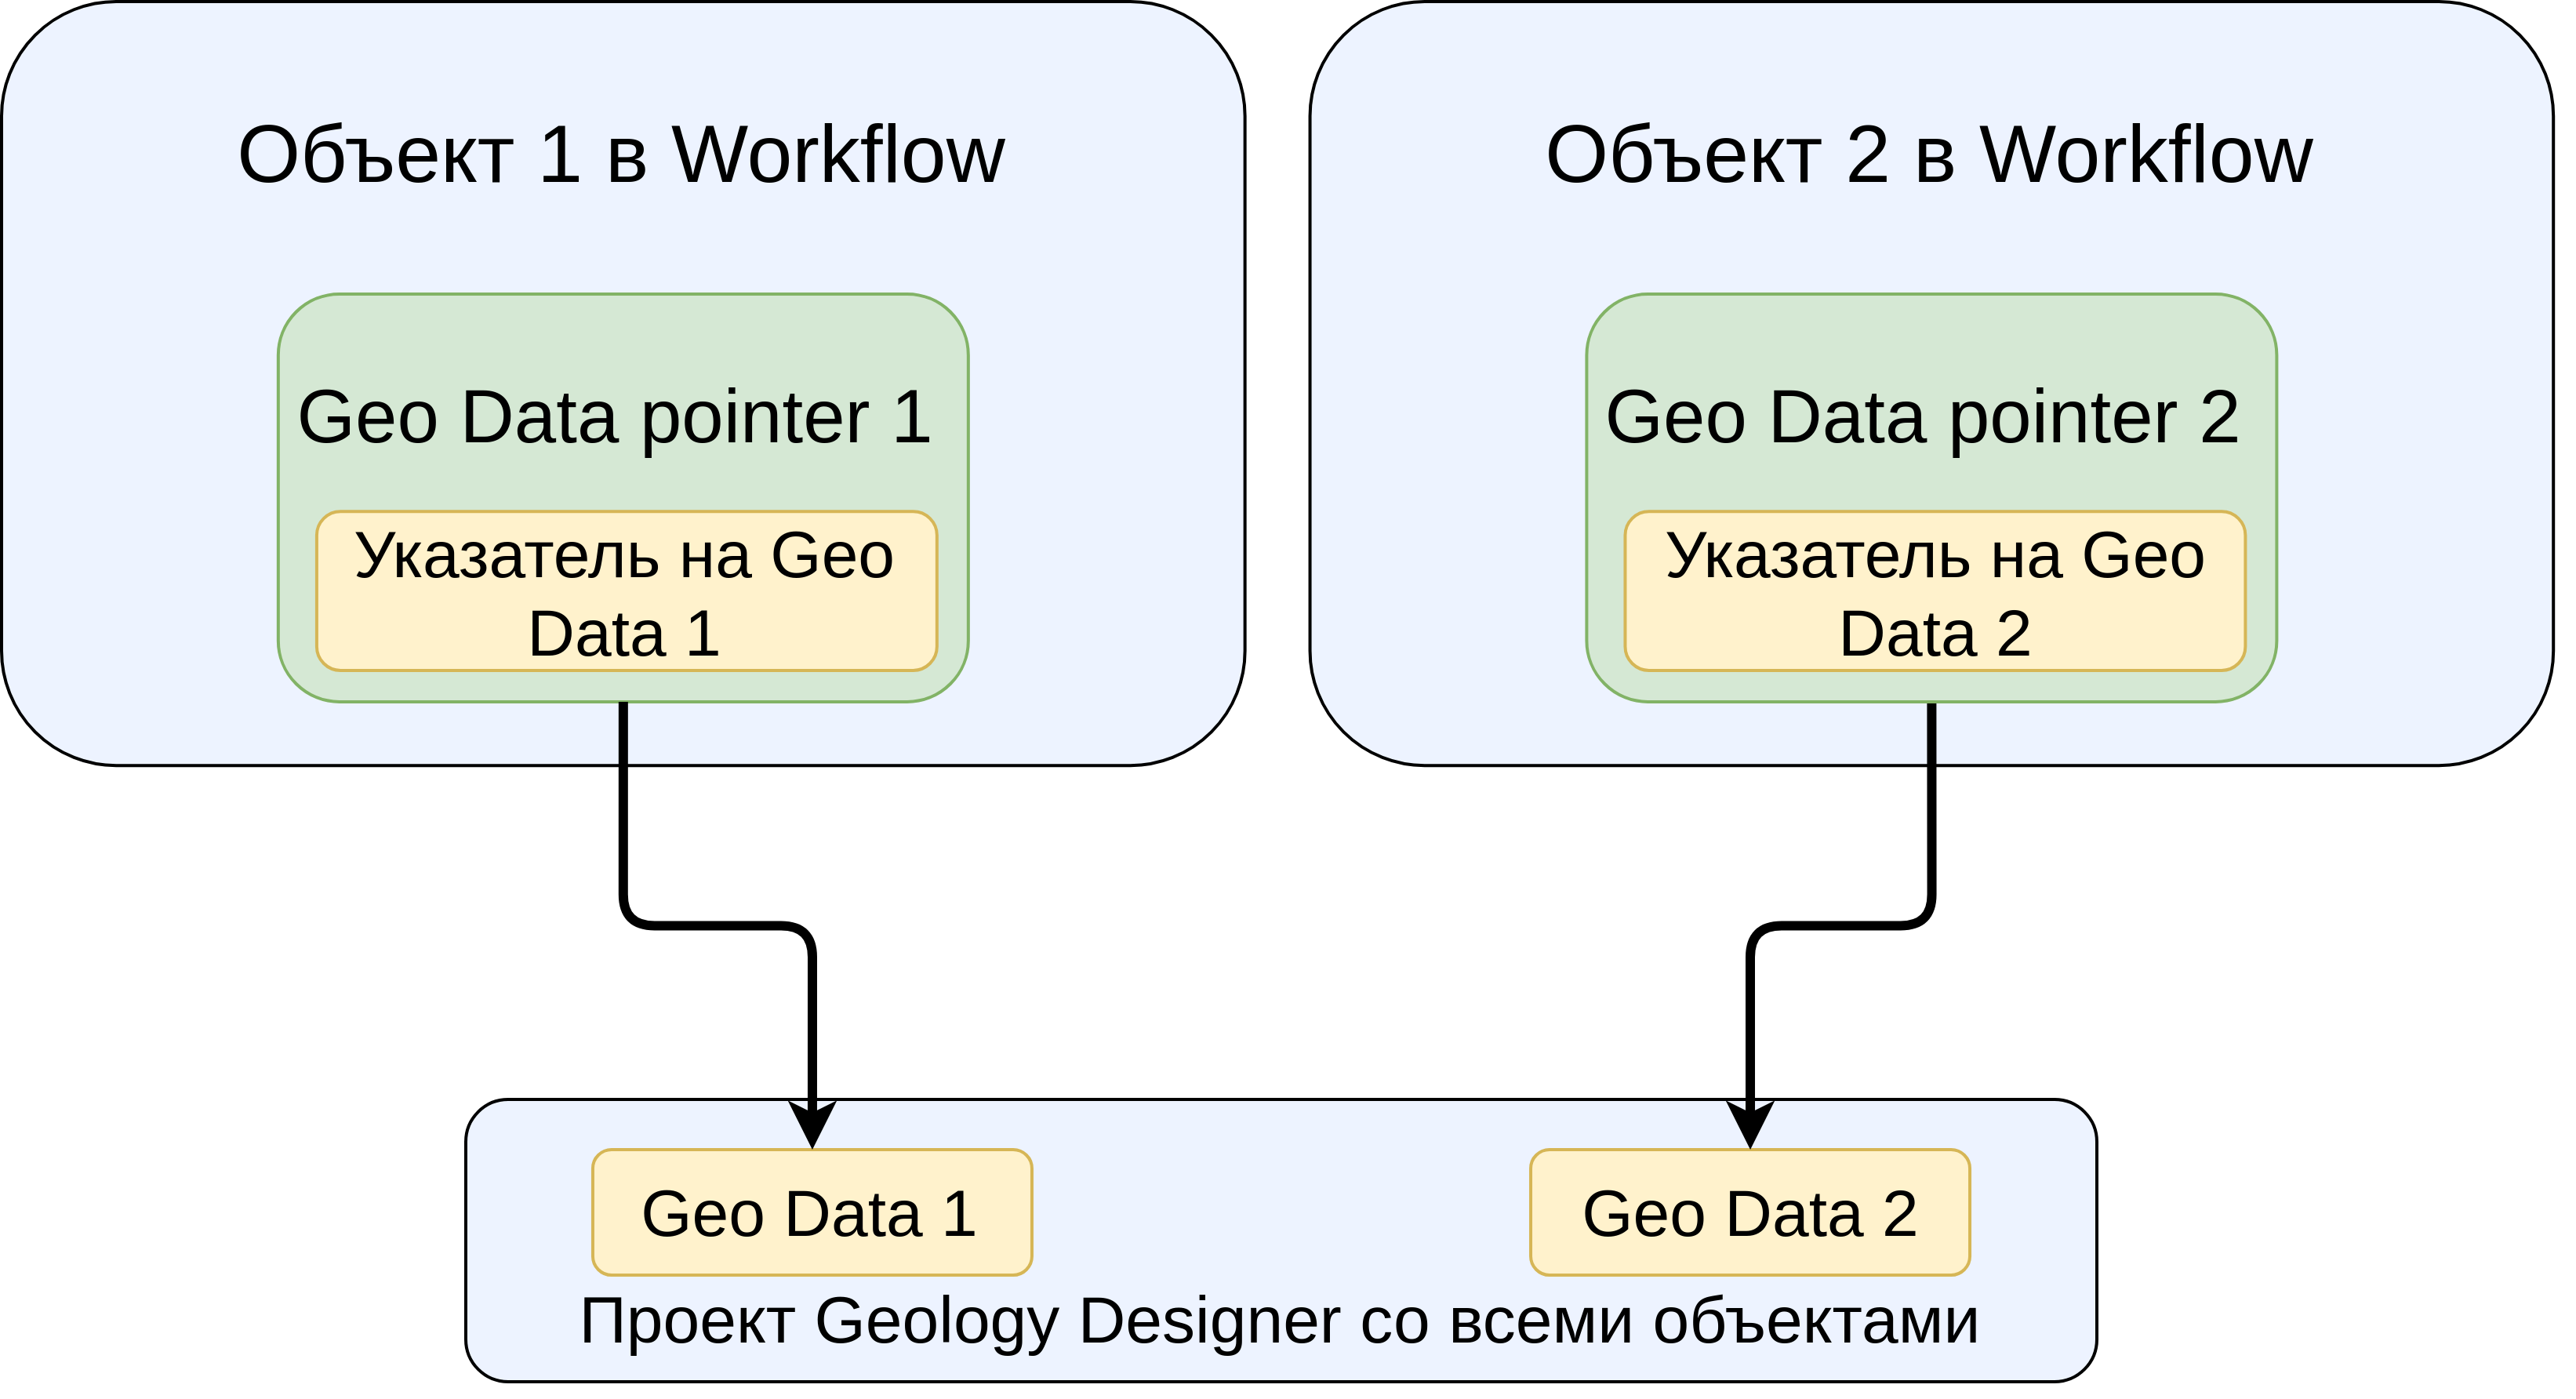
\includegraphics [width=460pt]{pics/object_logic_after.png}}
	\caption{Новая логика хранения объектов в Workflow}
\end{figure}


